\documentclass[
	classe=$1^{ere}STI2D$,
]{coursclass}

\title{Chapitre 4 : Polynômes de degré 2 et 3}
\date{}

\begin{document}

\maketitle

\begin{definition}[Polynôme de degré 2]
	Une \textbf{fonction polynôme de degré 2} est une fonction pouvant s'écrire sous la forme
	$$ f(x) = ax² + bx + c $$
	Où $a$, $b$ et $c$ sont des nombres constants.
\end{definition}

\begin{definition}[Racines]
	Une fonction de degré 2 peut \textit{parfois} (mais pas tout le temps) s'écrire sous la forme
	$$ f(x) = a × (x - r₁) × (x - r₂) $$
	Dans ce cas, on dit que $r₁$ et $r₂$ sont les \textbf{racines} de $f$.
\end{definition}

\begin{exemple}
	Si on développe l'expression $(x + 2)(x - 1)$, on obtient $x² + x - 2$.

	On dit que la fonction $f(x) = x² + x - 2$ s'écrit aussi $f(x) = (x + 2)(x - 1)$, et a pour racines

	$-2$ et $1$.
\end{exemple}

\begin{propriete}
	Si $r₁$ et $r₂$ sont les racines d'une fonction de degré 2 $f$, on a $f(r₁) = f(r₂) = 0$.
\end{propriete}

\begin{figure}[h!]
	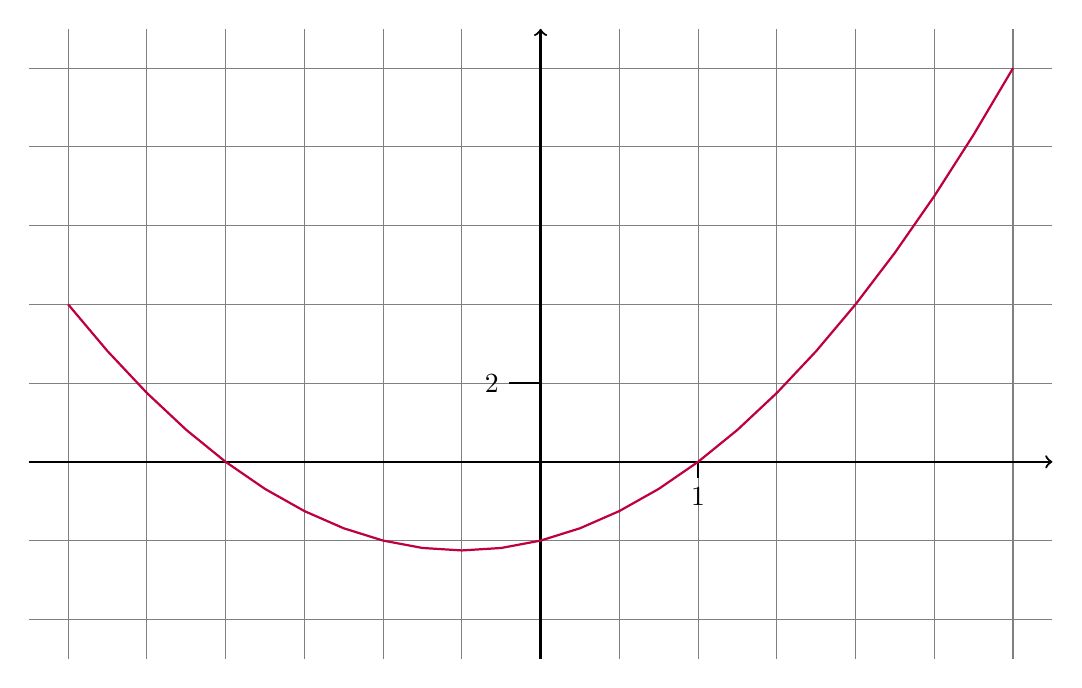
\begin{tikzpicture}[xscale=2]
		\draw[thin,gray,xstep=0.5] (-3.25,-2.5) grid (3.25,5.5);
		\draw[thick,->] (-3.25,0) -- (3.25,0);
		\draw[thick,->] (0,-2.5) -- (0,5.5);
		\draw[thick] (1,0) -- ++(0,-0.2) node[below] {$1$}
		(0,1) -- ++(-0.2,0) node[left] {$2$};
		\draw[thick,purple,variable=\x,domain=-3:3] plot({\x},{0.5*(\x+2)*(\x-1)});
	\end{tikzpicture}
	\caption*{graphe de la fonction $f(x) = (x + 2) (x - 1)$}
\end{figure}

\begin{propriete}[Courbe d'une fonction de degré 2]
	Si $f(x) = ax² + bx + c$ est une fonction de degré $2$, on peut trouver certaines propriétés de sa courbe :
	\begin{itemize}
		\item Si $a > 0$, les "bras" de la courbe sont dirigés vers le haut. Sinon, ils sont dirigés vers le bas.
		\item Le point le plus bas (si $a > 0$) ou haut (si $a < 0$) de la courbe a pour abscisse $-\dfrac{b}{2a}$.
		\item La courbe est symétrique par rapport à l'axe $x = -\dfrac{b}{2a}$.
	\end{itemize}

	\medskip

	Si on a de plus la forme factorisée de la fonction $f(x) = a(x - r₁)(x - r₂)$, on sait que les points $ (r₁ ; 0) $ et $ (r₂ ; 0) $ font partie de la courbe.
\end{propriete}

\end{document}